% Options for packages loaded elsewhere
% Options for packages loaded elsewhere
\PassOptionsToPackage{unicode}{hyperref}
\PassOptionsToPackage{hyphens}{url}
\PassOptionsToPackage{dvipsnames,svgnames,x11names}{xcolor}
%
\documentclass[
  letterpaper,
]{article}
\usepackage{xcolor}
\usepackage{amsmath,amssymb}
\setcounter{secnumdepth}{5}
\usepackage{iftex}
\ifPDFTeX
  \usepackage[T1]{fontenc}
  \usepackage[utf8]{inputenc}
  \usepackage{textcomp} % provide euro and other symbols
\else % if luatex or xetex
  \usepackage{unicode-math} % this also loads fontspec
  \defaultfontfeatures{Scale=MatchLowercase}
  \defaultfontfeatures[\rmfamily]{Ligatures=TeX,Scale=1}
\fi
\usepackage{lmodern}
\ifPDFTeX\else
  % xetex/luatex font selection
\fi
% Use upquote if available, for straight quotes in verbatim environments
\IfFileExists{upquote.sty}{\usepackage{upquote}}{}
\IfFileExists{microtype.sty}{% use microtype if available
  \usepackage[]{microtype}
  \UseMicrotypeSet[protrusion]{basicmath} % disable protrusion for tt fonts
}{}
\makeatletter
\@ifundefined{KOMAClassName}{% if non-KOMA class
  \IfFileExists{parskip.sty}{%
    \usepackage{parskip}
  }{% else
    \setlength{\parindent}{0pt}
    \setlength{\parskip}{6pt plus 2pt minus 1pt}}
}{% if KOMA class
  \KOMAoptions{parskip=half}}
\makeatother
% Make \paragraph and \subparagraph free-standing
\makeatletter
\ifx\paragraph\undefined\else
  \let\oldparagraph\paragraph
  \renewcommand{\paragraph}{
    \@ifstar
      \xxxParagraphStar
      \xxxParagraphNoStar
  }
  \newcommand{\xxxParagraphStar}[1]{\oldparagraph*{#1}\mbox{}}
  \newcommand{\xxxParagraphNoStar}[1]{\oldparagraph{#1}\mbox{}}
\fi
\ifx\subparagraph\undefined\else
  \let\oldsubparagraph\subparagraph
  \renewcommand{\subparagraph}{
    \@ifstar
      \xxxSubParagraphStar
      \xxxSubParagraphNoStar
  }
  \newcommand{\xxxSubParagraphStar}[1]{\oldsubparagraph*{#1}\mbox{}}
  \newcommand{\xxxSubParagraphNoStar}[1]{\oldsubparagraph{#1}\mbox{}}
\fi
\makeatother

\usepackage{color}
\usepackage{fancyvrb}
\newcommand{\VerbBar}{|}
\newcommand{\VERB}{\Verb[commandchars=\\\{\}]}
\DefineVerbatimEnvironment{Highlighting}{Verbatim}{commandchars=\\\{\}}
% Add ',fontsize=\small' for more characters per line
\usepackage{framed}
\definecolor{shadecolor}{RGB}{241,243,245}
\newenvironment{Shaded}{\begin{snugshade}}{\end{snugshade}}
\newcommand{\AlertTok}[1]{\textcolor[rgb]{0.68,0.00,0.00}{#1}}
\newcommand{\AnnotationTok}[1]{\textcolor[rgb]{0.37,0.37,0.37}{#1}}
\newcommand{\AttributeTok}[1]{\textcolor[rgb]{0.40,0.45,0.13}{#1}}
\newcommand{\BaseNTok}[1]{\textcolor[rgb]{0.68,0.00,0.00}{#1}}
\newcommand{\BuiltInTok}[1]{\textcolor[rgb]{0.00,0.23,0.31}{#1}}
\newcommand{\CharTok}[1]{\textcolor[rgb]{0.13,0.47,0.30}{#1}}
\newcommand{\CommentTok}[1]{\textcolor[rgb]{0.37,0.37,0.37}{#1}}
\newcommand{\CommentVarTok}[1]{\textcolor[rgb]{0.37,0.37,0.37}{\textit{#1}}}
\newcommand{\ConstantTok}[1]{\textcolor[rgb]{0.56,0.35,0.01}{#1}}
\newcommand{\ControlFlowTok}[1]{\textcolor[rgb]{0.00,0.23,0.31}{\textbf{#1}}}
\newcommand{\DataTypeTok}[1]{\textcolor[rgb]{0.68,0.00,0.00}{#1}}
\newcommand{\DecValTok}[1]{\textcolor[rgb]{0.68,0.00,0.00}{#1}}
\newcommand{\DocumentationTok}[1]{\textcolor[rgb]{0.37,0.37,0.37}{\textit{#1}}}
\newcommand{\ErrorTok}[1]{\textcolor[rgb]{0.68,0.00,0.00}{#1}}
\newcommand{\ExtensionTok}[1]{\textcolor[rgb]{0.00,0.23,0.31}{#1}}
\newcommand{\FloatTok}[1]{\textcolor[rgb]{0.68,0.00,0.00}{#1}}
\newcommand{\FunctionTok}[1]{\textcolor[rgb]{0.28,0.35,0.67}{#1}}
\newcommand{\ImportTok}[1]{\textcolor[rgb]{0.00,0.46,0.62}{#1}}
\newcommand{\InformationTok}[1]{\textcolor[rgb]{0.37,0.37,0.37}{#1}}
\newcommand{\KeywordTok}[1]{\textcolor[rgb]{0.00,0.23,0.31}{\textbf{#1}}}
\newcommand{\NormalTok}[1]{\textcolor[rgb]{0.00,0.23,0.31}{#1}}
\newcommand{\OperatorTok}[1]{\textcolor[rgb]{0.37,0.37,0.37}{#1}}
\newcommand{\OtherTok}[1]{\textcolor[rgb]{0.00,0.23,0.31}{#1}}
\newcommand{\PreprocessorTok}[1]{\textcolor[rgb]{0.68,0.00,0.00}{#1}}
\newcommand{\RegionMarkerTok}[1]{\textcolor[rgb]{0.00,0.23,0.31}{#1}}
\newcommand{\SpecialCharTok}[1]{\textcolor[rgb]{0.37,0.37,0.37}{#1}}
\newcommand{\SpecialStringTok}[1]{\textcolor[rgb]{0.13,0.47,0.30}{#1}}
\newcommand{\StringTok}[1]{\textcolor[rgb]{0.13,0.47,0.30}{#1}}
\newcommand{\VariableTok}[1]{\textcolor[rgb]{0.07,0.07,0.07}{#1}}
\newcommand{\VerbatimStringTok}[1]{\textcolor[rgb]{0.13,0.47,0.30}{#1}}
\newcommand{\WarningTok}[1]{\textcolor[rgb]{0.37,0.37,0.37}{\textit{#1}}}

\usepackage{longtable,booktabs,array}
\newcounter{none} % for unnumbered tables
\usepackage{calc} % for calculating minipage widths
% Correct order of tables after \paragraph or \subparagraph
\usepackage{etoolbox}
\makeatletter
\patchcmd\longtable{\par}{\if@noskipsec\mbox{}\fi\par}{}{}
\makeatother
% Allow footnotes in longtable head/foot
\IfFileExists{footnotehyper.sty}{\usepackage{footnotehyper}}{\usepackage{footnote}}
\makesavenoteenv{longtable}
\usepackage{graphicx}
\makeatletter
\newsavebox\pandoc@box
\newcommand*\pandocbounded[1]{% scales image to fit in text height/width
  \sbox\pandoc@box{#1}%
  \Gscale@div\@tempa{\textheight}{\dimexpr\ht\pandoc@box+\dp\pandoc@box\relax}%
  \Gscale@div\@tempb{\linewidth}{\wd\pandoc@box}%
  \ifdim\@tempb\p@<\@tempa\p@\let\@tempa\@tempb\fi% select the smaller of both
  \ifdim\@tempa\p@<\p@\scalebox{\@tempa}{\usebox\pandoc@box}%
  \else\usebox{\pandoc@box}%
  \fi%
}
% Set default figure placement to htbp
\def\fps@figure{htbp}
\makeatother





\setlength{\emergencystretch}{3em} % prevent overfull lines

\providecommand{\tightlist}{%
  \setlength{\itemsep}{0pt}\setlength{\parskip}{0pt}}



 


\makeatletter
\@ifpackageloaded{caption}{}{\usepackage{caption}}
\AtBeginDocument{%
\ifdefined\contentsname
  \renewcommand*\contentsname{Table of contents}
\else
  \newcommand\contentsname{Table of contents}
\fi
\ifdefined\listfigurename
  \renewcommand*\listfigurename{List of Figures}
\else
  \newcommand\listfigurename{List of Figures}
\fi
\ifdefined\listtablename
  \renewcommand*\listtablename{List of Tables}
\else
  \newcommand\listtablename{List of Tables}
\fi
\ifdefined\figurename
  \renewcommand*\figurename{Figure}
\else
  \newcommand\figurename{Figure}
\fi
\ifdefined\tablename
  \renewcommand*\tablename{Table}
\else
  \newcommand\tablename{Table}
\fi
}
\@ifpackageloaded{float}{}{\usepackage{float}}
\floatstyle{ruled}
\@ifundefined{c@chapter}{\newfloat{codelisting}{h}{lop}}{\newfloat{codelisting}{h}{lop}[chapter]}
\floatname{codelisting}{Listing}
\newcommand*\listoflistings{\listof{codelisting}{List of Listings}}
\makeatother
\makeatletter
\makeatother
\makeatletter
\@ifpackageloaded{caption}{}{\usepackage{caption}}
\@ifpackageloaded{subcaption}{}{\usepackage{subcaption}}
\makeatother
\usepackage{bookmark}
\IfFileExists{xurl.sty}{\usepackage{xurl}}{} % add URL line breaks if available
\urlstyle{same}
\hypersetup{
  pdftitle={1º Desafio em Elementos de Aprendizado de Máquina},
  pdfauthor={Lorrayne Silva; Kammyla Landim; Paulo Emílio Vaz},
  colorlinks=true,
  linkcolor={blue},
  filecolor={Maroon},
  citecolor={Blue},
  urlcolor={Blue},
  pdfcreator={LaTeX via pandoc}}


\title{1º Desafio em Elementos de Aprendizado de Máquina}
\usepackage{etoolbox}
\makeatletter
\providecommand{\subtitle}[1]{% add subtitle to \maketitle
  \apptocmd{\@title}{\par {\large #1 \par}}{}{}
}
\makeatother
\subtitle{Exercício 1 - ANEEL e Exercício 2 - Dataset Danish Lung
Cancer}
\author{Lorrayne Silva \and Kammyla Landim \and Paulo Emílio Vaz}
\date{2026-05-11}
\begin{document}
\maketitle

\renewcommand*\contentsname{Table of contents}
{
\setcounter{tocdepth}{3}
\tableofcontents
}

\section{Exercício 1}\label{exercuxedcio-1}

\subsection{Regressão Linear Múltipla - Eficiência Operacional
(ANEEL)}\label{regressuxe3o-linear-muxfaltipla---eficiuxeancia-operacional-aneel}

\#\#Nesta etapa, o nosso objetivo é avaliar se os Custos Operacionais
(PMSO) das 52 distribuidoras de energia podem ser explicados pelas suas
características operacionais (tamanho da rede, mercado, perdas, etc.).

\#\#Buscamos o melhor modelo de Regressão Linear Múltipla, equilibrando
a capacidade preditiva e a simplicidade interpretativa. Para isso, as
variáveis de identificação das empresas (DMU e Código) serão
desconsideradas da modelagem.

\subsubsection{1.1 Carga e Preparação dos
Dados}\label{carga-e-preparauxe7uxe3o-dos-dados}

\begin{Shaded}
\begin{Highlighting}[]
\DocumentationTok{\#\# Exercício 1: Regressão Linear Múltipla {-} Eficiência Operacional (ANEEL)}

\DocumentationTok{\#\#Nesta etapa, o nosso objetivo é avaliar se os Custos Operacionais (PMSO) das 52 distribuidoras de energia podem ser explicados pelas suas características operacionais (tamanho da rede, mercado, perdas, etc.). }

\DocumentationTok{\#\#Buscamos o melhor modelo de Regressão Linear Múltipla, equilibrando a capacidade preditiva e a simplicidade interpretativa. Para isso, as variáveis de identificação das empresas (DMU e Código) serão desconsideradas da modelagem.}

\DocumentationTok{\#\#\# 1.1 Carga e Preparação dos Dados}
\end{Highlighting}
\end{Shaded}

\begin{Shaded}
\begin{Highlighting}[]
\CommentTok{\# Carregando o pacote para leitura de planilhas}
\FunctionTok{library}\NormalTok{(readxl)}

\CommentTok{\# Lendo a base de dados}
\NormalTok{dados\_aneel }\OtherTok{\textless{}{-}} \FunctionTok{read\_excel}\NormalTok{(}\StringTok{"ModeloVigente\_DadosCP62\_2023.xlsx"}\NormalTok{)}

\CommentTok{\# Visualizando a estrutura inicial dos dados}
\FunctionTok{head}\NormalTok{(dados\_aneel)}
\end{Highlighting}
\end{Shaded}

\begin{verbatim}
# A tibble: 6 x 10
  DMU         Codigo   PMSO `rede alta` `rede subterranea` `rede aerea` mercadoP
  <chr>       <chr>   <dbl>       <dbl>              <dbl>        <dbl>    <dbl>
1 RGE SUL (F~ D01f   8.73e5       4316.            73.3         152713. 8369799.
2 AMAZONAS    D02    8.11e5        251.            36.7          35968. 2758709.
3 ENEL RJ     D03    7.80e5       3666.          3284.           54738. 5618601.
4 BANDEIRANTE D04    4.74e5       1034.           220.           28193. 5300379.
5 BOA VISTA ~ D05    1.62e5        713.             0.0500       16307.  642847.
6 ESS (FUSAO~ D06f   2.26e5        504.          1051.           30826. 2286742.
# i 3 more variables: cons <dbl>, CHI <dbl>, PNT <dbl>
\end{verbatim}

\textbf{1.2. Ajuste do Modelo Completo (Regressão Linear Múltipla):} Nós
iniciamos aplicando a Regressão Linear Múltipla clássica inserindo todas
as variáveis explicativas disponíveis (excluindo apenas os
identificadores textuais, como já discutimos). O objetivo foi criar uma
``linha de base'' para entender como todas as forças atuavam juntas
sobre o Custo Operacional (PMSO).

\begin{Shaded}
\begin{Highlighting}[]
\CommentTok{\# Ajustando o modelo completo (Prevendo PMSO e ignorando DMU e Codigo)}
\NormalTok{modelo\_completo }\OtherTok{\textless{}{-}} \FunctionTok{lm}\NormalTok{(PMSO }\SpecialCharTok{\textasciitilde{}}\NormalTok{ . }\SpecialCharTok{{-}}\NormalTok{ DMU }\SpecialCharTok{{-}}\NormalTok{ Codigo, }\AttributeTok{data =}\NormalTok{ dados\_aneel)}

\CommentTok{\# Visualizando os resultados do modelo completo}
\FunctionTok{summary}\NormalTok{(modelo\_completo)}
\end{Highlighting}
\end{Shaded}

\begin{verbatim}

Call:
lm(formula = PMSO ~ . - DMU - Codigo, data = dados_aneel)

Residuals:
    Min      1Q  Median      3Q     Max 
-195964  -27080  -17861   30823  224701 

Coefficients:
                     Estimate Std. Error t value Pr(>|t|)    
(Intercept)         2.171e+04  1.569e+04   1.384  0.17334    
`rede alta`        -3.937e+01  1.651e+01  -2.384  0.02148 *  
`rede subterranea`  2.147e+01  1.997e+01   1.075  0.28824    
`rede aerea`        2.896e+00  5.632e-01   5.142 6.02e-06 ***
mercadoP            3.662e-02  1.069e-02   3.426  0.00134 ** 
cons                9.304e-02  3.397e-02   2.739  0.00886 ** 
CHI                 3.484e-04  1.780e-03   0.196  0.84572    
PNT                 1.914e-01  3.543e-02   5.403 2.52e-06 ***
---
Signif. codes:  0 '***' 0.001 '**' 0.01 '*' 0.05 '.' 0.1 ' ' 1

Residual standard error: 82120 on 44 degrees of freedom
Multiple R-squared:  0.9798,    Adjusted R-squared:  0.9766 
F-statistic: 304.9 on 7 and 44 DF,  p-value: < 2.2e-16
\end{verbatim}

\textbf{1.3. Análise da Relevância Estatística (Modelo Completo):} No
caso do CHI e da Rede Subterrânea, o p-valor ficou muito acima do nível
de significância de 0,05 (0,84 e 0,28, respectivamente). Isso significa
que a probabilidade de estarmos observando essa relação apenas por acaso
(ruído dos dados) é alta demais. Como o nível de dúvida superou nosso
limite de segurança, falhamos em rejeitar a hipótese nula. Portanto,
concluímos que não há evidências estatísticas de que essas variáveis
impactem os custos operacionais e decidimos excluí-las para manter o
modelo parcimonioso e confiável.

No sumário acima, é possível identificar que as outras variáveis passam
no teste de significância, sendo que a PNT e a Rede Aérea são as que
apresentam o maior grau de significância estatística (p \textless{}
0,001, indicados pelos códigos visuais \texttt{***}).

No bloco seguinte, removemos manualmente as variáveis não significativas
e validamos essa escolha através do teste de diferença de Deviance
(ANOVA), conforme a metodologia apresentada na Aula 03 (Slide 3).

\begin{Shaded}
\begin{Highlighting}[]
\CommentTok{\# Ajustando o modelo reduzido (removendo \textquotesingle{}rede subterranea\textquotesingle{} e \textquotesingle{}CHI\textquotesingle{})}
\NormalTok{modelo\_reduzido }\OtherTok{\textless{}{-}} \FunctionTok{lm}\NormalTok{(PMSO }\SpecialCharTok{\textasciitilde{}} \StringTok{\textasciigrave{}}\AttributeTok{rede alta}\StringTok{\textasciigrave{}} \SpecialCharTok{+} \StringTok{\textasciigrave{}}\AttributeTok{rede aerea}\StringTok{\textasciigrave{}} \SpecialCharTok{+}\NormalTok{ mercadoP }\SpecialCharTok{+}\NormalTok{ cons }\SpecialCharTok{+}\NormalTok{ PNT, }
                      \AttributeTok{data =}\NormalTok{ dados\_aneel)}

\CommentTok{\# Resumo do modelo reduzido}
\FunctionTok{summary}\NormalTok{(modelo\_reduzido)}
\end{Highlighting}
\end{Shaded}

\begin{verbatim}

Call:
lm(formula = PMSO ~ `rede alta` + `rede aerea` + mercadoP + cons + 
    PNT, data = dados_aneel)

Residuals:
    Min      1Q  Median      3Q     Max 
-194771  -26642  -17927   29080  219176 

Coefficients:
               Estimate Std. Error t value Pr(>|t|)    
(Intercept)   2.197e+04  1.510e+04   1.455  0.15247    
`rede alta`  -3.809e+01  1.604e+01  -2.374  0.02180 *  
`rede aerea`  2.761e+00  5.200e-01   5.310 3.09e-06 ***
mercadoP      3.431e-02  1.033e-02   3.321  0.00176 ** 
cons          1.076e-01  3.081e-02   3.491  0.00107 ** 
PNT           2.025e-01  3.290e-02   6.155 1.69e-07 ***
---
Signif. codes:  0 '***' 0.001 '**' 0.01 '*' 0.05 '.' 0.1 ' ' 1

Residual standard error: 81380 on 46 degrees of freedom
Multiple R-squared:  0.9793,    Adjusted R-squared:  0.977 
F-statistic: 434.3 on 5 and 46 DF,  p-value: < 2.2e-16
\end{verbatim}

\begin{Shaded}
\begin{Highlighting}[]
\CommentTok{\# Comparação de Desvios (Deviance / ANOVA)}
\FunctionTok{anova}\NormalTok{(modelo\_reduzido, modelo\_completo)}
\end{Highlighting}
\end{Shaded}

\begin{verbatim}
Analysis of Variance Table

Model 1: PMSO ~ `rede alta` + `rede aerea` + mercadoP + cons + PNT
Model 2: PMSO ~ (DMU + Codigo + `rede alta` + `rede subterranea` + `rede aerea` + 
    mercadoP + cons + CHI + PNT) - DMU - Codigo
  Res.Df        RSS Df  Sum of Sq      F Pr(>F)
1     46 3.0467e+11                            
2     44 2.9670e+11  2 7972199165 0.5911  0.558
\end{verbatim}

\textbf{1.4 Seleção de Variáveis e Capacidade Preditiva:}

Para obter o novo modelo acima, removemos manualmente as variáveis não
significativas. Para validar essa remoção, aplicamos o teste de Análise
de Variância (ANOVA), que avalia a diferença de desvios (Deviance) entre
os dois modelos.

O teste ANOVA retornou um valor-p alto (p \textgreater{} 0.05), o que
indica que a remoção das variáveis ``Rede Subterrânea'' e ``CHI'' não
causou uma perda significativa de qualidade no ajuste. Como o p-valor do
modelo ficou em 0,558 não rejeitamos a hipótese nula (os dois modelos
são iguais em capacidade de explicação , ou seja as variáveis que
retiramos não fazem falta).

O \texttt{modelo\_reduzido} final atende aos objetivos do desafio:

\begin{enumerate}
\def\labelenumi{\arabic{enumi}.}
\item
  \textbf{Relevância:} Todas as variáveis mantidas (Rede de alta tensão,
  Rede aérea, Mercado, Consumidores e PNT) são altamente significativas
  (p \textless{} 0.05).
\item
  \textbf{Capacidade Preditiva:} O modelo reteve um \(R^2\) Ajustado de
  0.977, demonstrando que 97,7\% da variação nos custos (PMSO) é
  perfeitamente explicada por este conjunto reduzido de variáveis
  operacionais.
\end{enumerate}

\begin{Shaded}
\begin{Highlighting}[]
\CommentTok{\# Dividindo a área de plotagem para mostrar 4 gráficos simultaneamente}
\FunctionTok{par}\NormalTok{(}\AttributeTok{mfrow =} \FunctionTok{c}\NormalTok{(}\DecValTok{2}\NormalTok{, }\DecValTok{2}\NormalTok{))}

\CommentTok{\# Plotando os gráficos de diagnóstico para o modelo escolhido}
\FunctionTok{plot}\NormalTok{(modelo\_reduzido)}
\end{Highlighting}
\end{Shaded}

\begin{center}
\pandocbounded{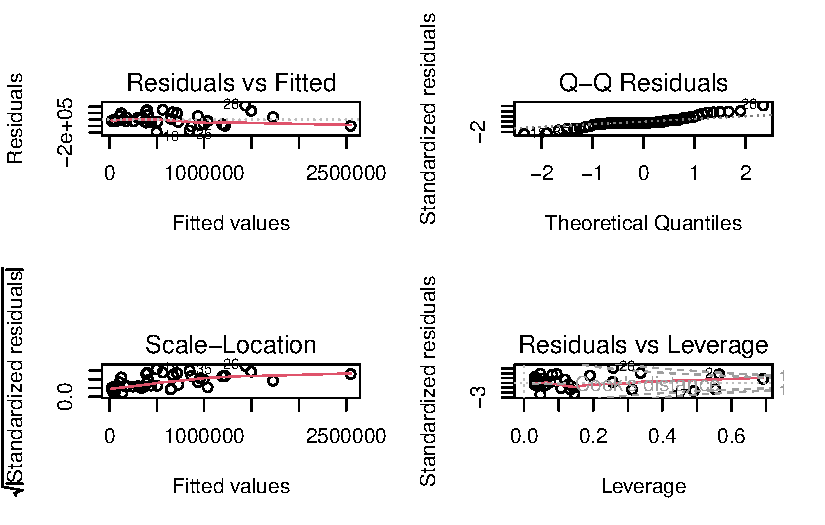
\includegraphics[keepaspectratio]{Desafio01_files/figure-pdf/unnamed-chunk-5-1.pdf}}
\end{center}

\begin{Shaded}
\begin{Highlighting}[]
\CommentTok{\# Retornando a área de plotagem ao padrão original}
\FunctionTok{par}\NormalTok{(}\AttributeTok{mfrow =} \FunctionTok{c}\NormalTok{(}\DecValTok{1}\NormalTok{, }\DecValTok{1}\NormalTok{))}
\end{Highlighting}
\end{Shaded}

\textbf{1.5 Principais Conclusões (Exercício 1):}

A partir do modelo reduzido selecionado, concluímos que é perfeitamente
viável para a ANEEL estimar os Custos Operacionais (PMSO) utilizando os
dados técnicos e de mercado das concessionárias. O modelo revelou que
97,7\% da variação desses custos é explicada por apenas cinco
variáveis-chave: Rede de alta tensão, Rede aérea, Mercado ponderado,
Consumidores e Perdas Não Técnicas (PNT).

Por outro lado, variáveis como ``Rede Subterrânea'' e ``CHI'' provaram
ser irrelevantes para a formação do custo operacional neste conjunto de
dados estatísticos. Esta descoberta é de alto valor para a ANEEL, pois
permite à agência focar seus esforços de regulação, auditoria e previsão
estritamente nas métricas que possuem impacto financeiro matematicamente
comprovado.

\section{Exercício 2}\label{exercuxedcio-2}

\textbf{2.1 Carga, Preparação e Análise Descritiva dos Dados:}

\begin{Shaded}
\begin{Highlighting}[]
\CommentTok{\# Criando o data frame com os dados do desafio}
\NormalTok{danishlc }\OtherTok{\textless{}{-}} \FunctionTok{data.frame}\NormalTok{(}
  \AttributeTok{City =} \FunctionTok{rep}\NormalTok{(}\FunctionTok{c}\NormalTok{(}\StringTok{"Fredericia"}\NormalTok{, }\StringTok{"Horsens"}\NormalTok{, }\StringTok{"Kolding"}\NormalTok{, }\StringTok{"Vejle"}\NormalTok{), }\AttributeTok{each =} \DecValTok{5}\NormalTok{),}
  \AttributeTok{Age =} \FunctionTok{rep}\NormalTok{(}\FunctionTok{c}\NormalTok{(}\StringTok{"40{-}54"}\NormalTok{, }\StringTok{"55{-}59"}\NormalTok{, }\StringTok{"60{-}64"}\NormalTok{, }\StringTok{"65{-}74"}\NormalTok{, }\StringTok{"\textgreater{}74"}\NormalTok{), }\AttributeTok{times =} \DecValTok{4}\NormalTok{),}
  \AttributeTok{Pop =} \FunctionTok{c}\NormalTok{(}\DecValTok{3059}\NormalTok{, }\DecValTok{800}\NormalTok{, }\DecValTok{710}\NormalTok{, }\DecValTok{581}\NormalTok{, }\DecValTok{509}\NormalTok{,  }
          \DecValTok{3083}\NormalTok{, }\DecValTok{712}\NormalTok{, }\DecValTok{625}\NormalTok{, }\DecValTok{402}\NormalTok{, }\DecValTok{290}\NormalTok{,  }
          \DecValTok{2867}\NormalTok{, }\DecValTok{597}\NormalTok{, }\DecValTok{526}\NormalTok{, }\DecValTok{350}\NormalTok{, }\DecValTok{223}\NormalTok{,  }
          \DecValTok{2914}\NormalTok{, }\DecValTok{539}\NormalTok{, }\DecValTok{461}\NormalTok{, }\DecValTok{307}\NormalTok{, }\DecValTok{189}\NormalTok{),}
  \AttributeTok{Cases =} \FunctionTok{c}\NormalTok{(}\DecValTok{11}\NormalTok{, }\DecValTok{11}\NormalTok{, }\DecValTok{11}\NormalTok{, }\DecValTok{10}\NormalTok{, }\DecValTok{11}\NormalTok{,  }
            \DecValTok{15}\NormalTok{, }\DecValTok{6}\NormalTok{, }\DecValTok{8}\NormalTok{, }\DecValTok{7}\NormalTok{, }\DecValTok{4}\NormalTok{,  }
            \DecValTok{11}\NormalTok{, }\DecValTok{13}\NormalTok{, }\DecValTok{9}\NormalTok{, }\DecValTok{11}\NormalTok{, }\DecValTok{10}\NormalTok{,  }
            \DecValTok{10}\NormalTok{, }\DecValTok{8}\NormalTok{, }\DecValTok{7}\NormalTok{, }\DecValTok{10}\NormalTok{, }\DecValTok{14}\NormalTok{)}
\NormalTok{)}

\CommentTok{\# Convertendo as variáveis explicativas para fatores}
\NormalTok{danishlc}\SpecialCharTok{$}\NormalTok{City }\OtherTok{\textless{}{-}} \FunctionTok{as.factor}\NormalTok{(danishlc}\SpecialCharTok{$}\NormalTok{City)}
\NormalTok{danishlc}\SpecialCharTok{$}\NormalTok{Age }\OtherTok{\textless{}{-}} \FunctionTok{as.factor}\NormalTok{(danishlc}\SpecialCharTok{$}\NormalTok{Age)}

\CommentTok{\# Calculando a Taxa Bruta de Incidência (por 1.000 habitantes)}
\NormalTok{danishlc}\SpecialCharTok{$}\NormalTok{Taxa }\OtherTok{\textless{}{-}}\NormalTok{ (danishlc}\SpecialCharTok{$}\NormalTok{Cases }\SpecialCharTok{/}\NormalTok{ danishlc}\SpecialCharTok{$}\NormalTok{Pop) }\SpecialCharTok{*} \DecValTok{1000}

\CommentTok{\# Visualizando o sumário descritivo dos dados}
\FunctionTok{summary}\NormalTok{(danishlc)}
\end{Highlighting}
\end{Shaded}

\begin{verbatim}
         City      Age         Pop             Cases            Taxa       
 Fredericia:5   >74  :4   Min.   : 189.0   Min.   : 4.00   Min.   : 3.432  
 Horsens   :5   40-54:4   1st Qu.: 389.0   1st Qu.: 8.00   1st Qu.:11.707  
 Kolding   :5   55-59:4   Median : 560.0   Median :10.00   Median :15.339  
 Vejle     :5   60-64:4   Mean   : 987.2   Mean   : 9.85   Mean   :19.403  
                65-74:4   3rd Qu.: 734.0   3rd Qu.:11.00   3rd Qu.:21.652  
                          Max.   :3083.0   Max.   :15.00   Max.   :74.074  
\end{verbatim}

\begin{Shaded}
\begin{Highlighting}[]
\FunctionTok{library}\NormalTok{(ggplot2)}

\FunctionTok{ggplot}\NormalTok{(danishlc, }\FunctionTok{aes}\NormalTok{(}\AttributeTok{x =}\NormalTok{ Age, }\AttributeTok{y =}\NormalTok{ Taxa, }\AttributeTok{fill =}\NormalTok{ City)) }\SpecialCharTok{+}
  \FunctionTok{geom\_bar}\NormalTok{(}\AttributeTok{stat =} \StringTok{"identity"}\NormalTok{, }\AttributeTok{position =} \StringTok{"dodge"}\NormalTok{) }\SpecialCharTok{+}
  \FunctionTok{theme\_minimal}\NormalTok{() }\SpecialCharTok{+}
  \FunctionTok{labs}\NormalTok{(}
    \AttributeTok{title =} \StringTok{"Taxa de Incidência de Câncer de Pulmão por 1.000 Habitantes"}\NormalTok{,}
    \AttributeTok{x =} \StringTok{"Faixa Etária (Anos)"}\NormalTok{,}
    \AttributeTok{y =} \StringTok{"Casos por 1.000 Habitantes"}\NormalTok{,}
    \AttributeTok{fill =} \StringTok{"Cidade"}
\NormalTok{  ) }\SpecialCharTok{+}
  \FunctionTok{scale\_fill\_brewer}\NormalTok{(}\AttributeTok{palette =} \StringTok{"Set2"}\NormalTok{)}
\end{Highlighting}
\end{Shaded}

\begin{center}
\pandocbounded{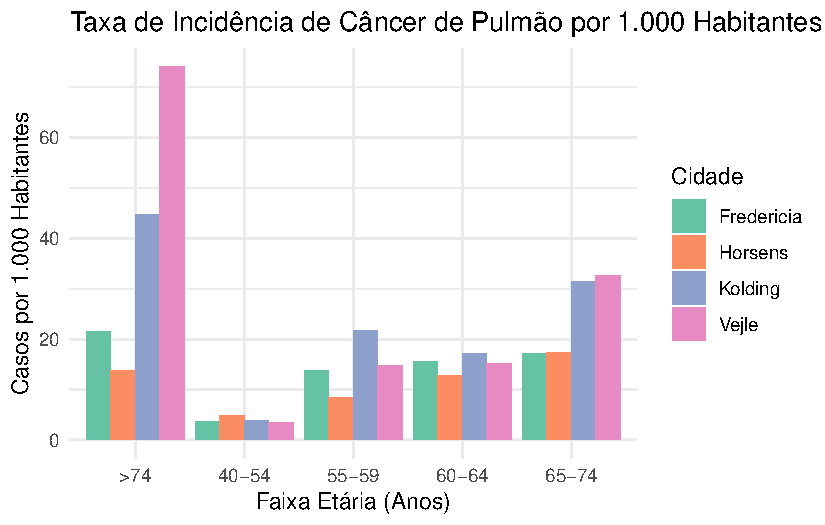
\includegraphics[keepaspectratio]{Desafio01_files/figure-pdf/unnamed-chunk-6-1.pdf}}
\end{center}

\textbf{2.2 Análise Descritiva:} A análise exploratória inicial da base
de dados revela o comportamento da taxa de incidência de câncer de
pulmão nas quatro cidades dinamarquesas observadas (Fredericia, Horsens,
Kolding e Vejle). Através da estatística descritiva e da visualização
gráfica, fica evidente que a taxa de incidência (casos por 1.000
habitantes) é assimetricamente maior na faixa etária mais avançada
(maiores de 74 anos), mantendo esse padrão de alta independentemente da
cidade analisada. Visualmente, as cidades de Kolding e Vejle já
demonstram barras mais elevadas nas idades mais críticas.

\begin{Shaded}
\begin{Highlighting}[]
\CommentTok{\# Ajustando o modelo de Poisson com offset populacional}
\NormalTok{modelo\_poisson }\OtherTok{\textless{}{-}} \FunctionTok{glm}\NormalTok{(}
\NormalTok{  Cases }\SpecialCharTok{\textasciitilde{}}\NormalTok{ City }\SpecialCharTok{+}\NormalTok{ Age, }
  \AttributeTok{family =} \FunctionTok{poisson}\NormalTok{(}\AttributeTok{link =} \StringTok{"log"}\NormalTok{), }
  \AttributeTok{offset =} \FunctionTok{log}\NormalTok{(Pop), }
  \AttributeTok{data =}\NormalTok{ danishlc}
\NormalTok{)}

\CommentTok{\# Exibindo os resultados detalhados do modelo}
\FunctionTok{summary}\NormalTok{(modelo\_poisson)}
\end{Highlighting}
\end{Shaded}

\begin{verbatim}

Call:
glm(formula = Cases ~ City + Age, family = poisson(link = "log"), 
    data = danishlc, offset = log(Pop))

Coefficients:
            Estimate Std. Error z value Pr(>|z|)    
(Intercept) -3.57882    0.19004 -18.832  < 2e-16 ***
CityHorsens -0.05664    0.20918  -0.271 0.786564    
CityKolding  0.40221    0.19339   2.080 0.037543 *  
CityVejle    0.39649    0.19865   1.996 0.045945 *  
Age40-54    -2.15918    0.21821  -9.895  < 2e-16 ***
Age55-59    -0.84403    0.22867  -3.691 0.000223 ***
Age60-64    -0.79328    0.23350  -3.397 0.000680 ***
Age65-74    -0.35432    0.22821  -1.553 0.120509    
---
Signif. codes:  0 '***' 0.001 '**' 0.01 '*' 0.05 '.' 0.1 ' ' 1

(Dispersion parameter for poisson family taken to be 1)

    Null deviance: 147.943  on 19  degrees of freedom
Residual deviance:  14.484  on 12  degrees of freedom
AIC: 112.55

Number of Fisher Scoring iterations: 4
\end{verbatim}

\begin{verbatim}
#| message: false
#| warning: false

# Extraindo as razões de taxas (exponencial dos coeficientes)
razao_taxas <- exp(coef(modelo_poisson))

# Calculando os Intervalos de Confiança (95%)
ic_razao_taxas <- exp(confint(modelo_poisson))

# Consolidando os resultados em uma tabela
tabela_interpretacao <- cbind(
  `Razão de Taxas (RR)` = razao_taxas, 
  ic_razao_taxas
)

print(round(tabela_interpretacao, 4))}
\end{verbatim}

\begin{verbatim}
#| message: false
#| warning: false

# Extraindo estatísticas de ajuste
deviance_residual <- modelo_poisson$deviance
graus_liberdade <- modelo_poisson$df.residual

# Calculando o p-valor do teste Qui-Quadrado
p_valor_ajuste <- pchisq(deviance_residual, df = graus_liberdade, lower.tail = FALSE)

cat("Deviance Residual:", round(deviance_residual, 4), "\n")
cat("Graus de Liberdade:", graus_liberdade, "\n")
cat("P-valor do Teste de Ajuste:", round(p_valor_ajuste, 4), "\n")
\end{verbatim}

\textbf{2.3 Ajuste do Modelo e Qualidade:}

Para modelar as contagens de casos da doença, aplicamos a Regressão de
Poisson com a função de ligação logarítmica. O passo fundamental neste
ajuste foi a utilização do logaritmo da População
(\texttt{offset\ =\ log(Pop)}). Na modelagem epidemiológica, o
\emph{offset} transforma a simples contagem bruta de casos em uma
\textbf{taxa de incidência}, permitindo uma comparação justa entre
cidades que possuem tamanhos populacionais diferentes.

O modelo demonstrou um excelente ajuste aos dados empíricos. Ao calcular
a \emph{Deviance Residual} (14,484 para 12 graus de liberdade) e
submetê-la ao teste de Qualidade de Ajuste (Qui-Quadrado), obtivemos um
p-valor amplamente superior ao nível de significância de 0,05. Esse
resultado nos leva a não rejeitar a hipótese nula de bom ajuste do
modelo, o que atesta a ausência de superdispersão e confirma que a
distribuição de Poisson foi a escolha metodológica correta.

\begin{Shaded}
\begin{Highlighting}[]
\CommentTok{\# Dividindo a área de plotagem para mostrar 4 gráficos simultaneamente}
\FunctionTok{par}\NormalTok{(}\AttributeTok{mfrow =} \FunctionTok{c}\NormalTok{(}\DecValTok{2}\NormalTok{, }\DecValTok{2}\NormalTok{))}

\CommentTok{\# Plotando os gráficos de diagnóstico para o modelo de Poisson}
\FunctionTok{plot}\NormalTok{(modelo\_poisson)}
\end{Highlighting}
\end{Shaded}

\begin{center}
\pandocbounded{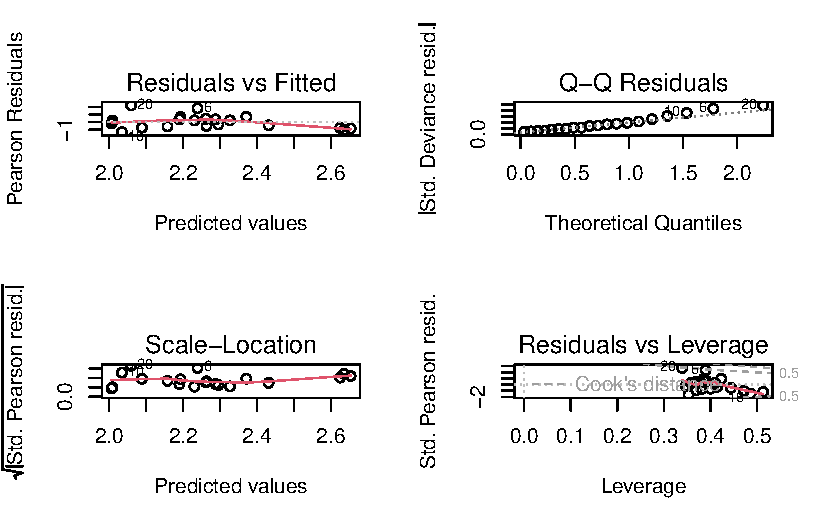
\includegraphics[keepaspectratio]{Desafio01_files/figure-pdf/unnamed-chunk-8-1.pdf}}
\end{center}

\begin{Shaded}
\begin{Highlighting}[]
\CommentTok{\# Retornando a área de plotagem ao padrão original}
\FunctionTok{par}\NormalTok{(}\AttributeTok{mfrow =} \FunctionTok{c}\NormalTok{(}\DecValTok{1}\NormalTok{, }\DecValTok{1}\NormalTok{))}
\end{Highlighting}
\end{Shaded}

\textbf{2.4 Análise dos Resíduos:}

A análise gráfica dos resíduos deviance confirma a adequação do modelo.
O gráfico Residuals vs Fitted não apresenta funilamento
(homocedasticidade respeitada), o que é corroborado pelo teste formal de
qualidade de ajuste (Qui-quadrado) realizado anteriormente, que
descartou a presença de superdispersão. Além disso, a ausência de pontos
que extrapolem a Distância de Cook no gráfico Residuals vs Leverage
indica que não há outliers influentes distorcendo as estimativas das
taxas de incidência nas cidades.

\textbf{2.5 Principais Conclusões:}

Com base nas Razões de Taxas (RR - Rate Ratios) extraídas da
exponenciação dos coeficientes do modelo, podemos caracterizar o perfil
de incidência do câncer de pulmão da seguinte forma:

Efeito da Idade: A idade é o fator de risco mais expressivo. Tomando a
faixa de maiores de 74 anos como base, observa-se que as taxas de
incidência caem drasticamente nas faixas mais jovens. Pacientes entre
40-54 anos, por exemplo, apresentam uma taxa de incidência cerca de 88\%
menor (RR = 0,11) quando comparados aos idosos (\textgreater74 anos). A
incidência cresce progressivamente conforme a idade avança.

Efeito da Localidade (Cidades): Tendo a cidade de Fredericia como
referência (linha de base do modelo), notamos que a cidade de Horsens
não apresenta diferença estatística significativa nas taxas (p
\textgreater{} 0,05). No entanto, as cidades de Kolding e Vejle
apresentam as maiores taxas da doença, com incidências aproximadamente
49\% e 48\% maiores (RR = 1,49 e RR = 1,48, respectivamente) do que
Fredericia, mantendo-se a faixa etária constante.

Conclusão Geral: O modelo confirmou que o risco de câncer de pulmão nas
cidades dinamarquesas analisadas aumenta severamente com o
envelhecimento da população, e que existe uma concentração geográfica de
maior risco (maiores taxas) nas cidades de Kolding e Vejle.




\end{document}
